\documentclass{article}

\usepackage{icml2026}
\usepackage{amsmath}
\usepackage{amssymb}
\usepackage{booktabs}
\usepackage{graphicx}
\usepackage{multirow}
\usepackage{hyperref}
\usepackage{url}
\usepackage{enumitem}
\graphicspath{{assets/plots/}{assets/media/}}

\icmltitlerunning{SAGE-Mem: Write-Time Governance for Multimodal Agent Memory}

\begin{document}

\twocolumn[
\icmltitle{SAGE-Mem: Write-Time Governance for Multimodal Agent Memory Under Adversarial and Noisy Observations}

\begin{icmlauthorlist}
\icmlauthor{Anonymous Author}{}
\end{icmlauthorlist}

\icmlaffiliation{}{Anonymous Institution}

\begin{icmlkeywords}
multimodal agents, memory safety, prompt injection, adversarial robustness
\end{icmlkeywords}

\vskip 0.3in
]

\printAffiliationsAndNotice{}



\begin{abstract}
Long-horizon agents increasingly rely on persistent memory, but persistent memory is also a durable attack surface. An adversarial observation that is admitted into memory can later be retrieved, consolidated, and reused long after the original interaction has ended. Existing defenses for memory poisoning are predominantly retrieval-time: they try to rank or filter memories after contamination has already entered the store. This leaves the memory state itself polluted, increases retrieval noise, wastes context budget, and allows unsupported observations to harden into derived beliefs. We study \textbf{write-time governed multimodal memory} as a distinct robustness problem. We present \textbf{SAGE-Mem}, a memory layer that mediates admission, promotion, and retrieval through typed memory partitions (\texttt{evidence}, \texttt{belief}, \texttt{control}), sufficiency-gated evidence-to-belief promotion, source-conditioned trust, anomaly detection, consistency checks, and provenance-aware retrieval. We evaluate on two settings: (i) a controlled long-horizon benchmark based on LoCoMo-10 with multimodal adversarial injections, including Visual Prompt Injection (VPI) and noisy/missing-modality stress; and (ii) an adversarially augmented MM-BrowseComp observation-trace benchmark with VLM-backed image observations. Our primary metrics follow the memory lifecycle: attack write admission, attack belief formation, retrieval contamination, false-belief retrieval, and benign completion under attack (BCU). On LoCoMo-based benchmarks, SAGE-Mem consistently drives write admission and retrieval contamination to near-zero, including perfect suppression on the main suite and VPI-only setting, while remaining robust under noisy/missing multimodal inputs. SAGE-Mem trails retrieval-time baselines on clean and attacked QA utility, so the result is an integrity--utility tradeoff rather than overall dominance. MM-BrowseComp further shows that generic tool trust fails under realistic browsing attacks. An initial browsing-specific extension, \textbf{SAGE-Mem-Browse}, reduces attack admission, but remains vulnerable on the harder combined browser benchmark. We therefore introduce \textbf{SAGE-Mem-BrowseGuard}, a browser-specific write-time layer that combines structured browser claim typing with page-group anomaly signals and channel provenance, without relying on correction-language keywords. On the 194-case grouped MM-BrowseComp benchmark, SAGE-Mem-BrowseGuard achieves Write ASR=0.000 and Retrieval ASR=0.000 on the combined injection+adaptive attack track, while preserving near-clean utility (\texttt{BCU\_poison=0.1512} vs \texttt{BCU\_clean=0.1598}). A later semantic observation-group rerun preserves the same top-line result without changing the main mechanistic interpretation. The resulting picture is not “retrieval is obsolete,” but rather that \textbf{write-time governance is a necessary complement to retrieval-time filtering for multimodal agent memory}, especially when dependent multimodal evidence can masquerade as corroboration and browser-derived factual claims can bypass generic tool trust.
\end{abstract}

\section{Introduction}

Memory changes what an agent is. A stateless model can only be manipulated in the current context window; a stateful agent can be manipulated by altering the persistent memory that future reasoning depends on. This makes memory poisoning qualitatively different from ordinary prompt injection. Once a malicious observation is written, it can survive long after the original turn, reappear at retrieval time, distort later summaries, and occupy retrieval bandwidth that should have been reserved for grounded evidence.

This matters even more for multimodal agents. OCR text, image captions, browser outputs, and user/tool messages are not interchangeable evidence channels. A single adversarial image can produce both OCR output and a caption-like summary, creating the appearance of multi-source support despite both observations originating from the same underlying source. In other words, multimodal agreement is not always evidence of truth; it can also be evidence of \textbf{dependent corruption}.

The paper’s multimodal claim should therefore be read precisely. We are \textbf{not} claiming to solve full multimodal truth inference or general cross-modal fact verification. Our claim is narrower and, we believe, more important for deployed agents: persistent memory systems need principled rules for deciding when heterogeneous multimodal observations are safe to store, when they should remain weak evidence, and when apparent cross-modal agreement is merely duplicated corruption from a single source object.

Most prior memory-poisoning defenses attack the problem too late. Retrieval-time reliability scoring can reduce the chance that a poisoned item is selected, but it does not protect the persistent memory state itself. A memory system that accepts unsupported observations and merely hopes to filter them later incurs three long-run costs:

\begin{enumerate}
\item \textbf{State corruption:} the store contains observations that should never have been admitted.
\item \textbf{Retrieval burden:} reranking and filtering must repeatedly separate signal from contamination.
\item \textbf{Compounding distortion:} later summaries and derived beliefs may inherit unsupported content.
\end{enumerate}

We therefore study \textbf{write-time governance} as the primary mechanism, and evaluate it with \textbf{lifecycle metrics} rather than only downstream QA metrics. The question is not just whether a poisoned memory is retrieved at the end of the pipeline, but whether it is admitted at write time, whether it hardens into a belief, whether it later resurfaces, and how much benign utility is preserved under that regime.

\subsection{Why Write-Time Defense Is Distinct}

This distinction from retrieval-time defense should be explicit. Retrieval-time filtering and write-time governance solve related but non-identical problems.

Retrieval-time defense asks:
\begin{itemize}
\item given a possibly contaminated memory store,
\item which items should be surfaced to the model right now?
\end{itemize}

Write-time defense asks the harder systems question:
\begin{itemize}
\item which observations should be allowed to become persistent state at all?
\end{itemize}

The second problem is harder for three reasons.

\begin{enumerate}
\item \textbf{Partial observability at ingestion time.} At write time the system has less future context than it will have at retrieval time. It must decide under uncertainty whether a fresh observation is trustworthy enough to store.
\item \textbf{Memory-state externalities.} A false positive or false negative at write time has long-run effects: accepted noise can distort future summaries, crowd out useful evidence, and repeatedly tax retrieval. Retrieval-only methods do not undo those state changes.
\item \textbf{Multimodal dependence.} In multimodal agents, two observations may appear to corroborate each other while actually deriving from the same source object, such as OCR and caption outputs from one image. This creates false support before the retrieval stage is ever reached.
\end{enumerate}

These differences motivate our evaluation choice. A write-time defense should not be judged only by final QA utility or retrieval-time ASR, because those are downstream outcomes of a longer memory lifecycle. The write boundary, the belief boundary, and the retrieval boundary each expose different failure modes.

This also means that comparing SAGE-Mem to a retrieval-time system such as MMA is not a single-axis leaderboard comparison. MMA is designed to preserve and rank a broad memory store at retrieval time, which naturally favors immediate answer utility. SAGE-Mem is designed to keep unsupported observations out of durable memory, which naturally favors store integrity and may reject evidence that later would have helped a benign question. We therefore interpret the comparison as an \textbf{integrity--utility frontier}: the central question is whether write-time governance buys measurable memory-state integrity, and what utility cost that purchase entails.

\subsection{Hypotheses}

We frame the paper around five explicit hypotheses.

\begin{itemize}
\item \textbf{H1: Write-time governance hypothesis.}
\end{itemize}
Relative to retrieval-time filtering alone, a governed write boundary should reduce attack write admission and retrieval contamination on long-horizon multimodal memory tasks.

\begin{itemize}
\item \textbf{H2: Belief-formation hypothesis.}
\end{itemize}
Typed evidence-to-belief promotion should reduce the rate at which unsupported or adversarial observations harden into durable, answer-bearing memory.

\begin{itemize}
\item \textbf{H3: Dependent-evidence hypothesis.}
\end{itemize}
Multimodal attacks such as VPI exploit dependence between OCR and caption outputs from the same image; modeling those channels as dependent should improve robustness relative to consensus-style trust.

\begin{itemize}
\item \textbf{H4: Noise-calibration hypothesis.}
\end{itemize}
Under noisy or missing modalities, adaptive trust calibration should reduce over-quarantine relative to simpler write-time baselines while preserving low attack survival.

\begin{itemize}
\item \textbf{H5: Browsing-context prior hypothesis.}
\end{itemize}
Browsing-derived external tool text is not equivalent to trusted internal tool output. A source-context-sensitive write prior should reduce realistic web-style correction-language attacks without globally lowering trust in all tool outputs. In the paper, this extension is instantiated as \textbf{SAGE-Mem-Browse}. \textbf{Scope caveat:} the initial browsing-prior implementation uses a keyword regex whose vocabulary overlaps with the benchmark attack text by construction. The resulting success therefore holds only for correction-language-vocabulary adversaries, not for adversaries who paraphrase the same semantic intent without trigger words.

\begin{itemize}
\item \textbf{H6: Browsing-guard hypothesis.}
\end{itemize}
A browser-specific, vocabulary-agnostic write-time layer should maintain robustness against adaptive adversaries who evade the H5 keyword filter. In the current design, \textbf{SAGE-Mem-BrowseGuard} combines a structured browser claim gate for browser-sourced \texttt{qa\_answer} writes with secondary page-group anomaly signals and channel provenance. H6 should reduce ASR on paraphrased correction attacks (\texttt{fact\_overwrite\_adaptive}) while preserving clean BCU close to the SAGE-Mem-Browse level.
\textbf{Empirical result:} H6 is \textbf{fully supported} on the current benchmark. On the combined adversarial benchmark (\texttt{paper\_mmadv\_abr\_group\_v1}, n=194 cases, 388 attack write attempts including both correction-language and vocabulary-adaptive phrasings), SAGE-Mem-BrowseGuard achieves Write ASR=0.000, Retrieval=0.000, ASR=0.000, BCU\_poison=0.1512. The primary mechanism is the structured browser claim gate: browser-sourced \texttt{qa\_answer} writes are blocked at the content-type level rather than by vocabulary matching. The gate fires an average of 2.0 times per case, blocking all 388/388 attack writes. Secondary page-group anomaly checks fire on 0.622 writes per case on average, providing additional within-page outlier coverage. For comparison, SAGE-Mem-Browse admits 122/388 writes (Write ASR=0.314), which then drive retrieval contamination to 0.827 and BCU\_poison down to 0.0275.

The current empirical evidence strongly supports H1, H3, and H4 on LoCoMo-based settings, partially supports H2 through near-zero false-belief retrieval, supports H5 narrowly for correction-language vocabulary attacks with the co-design caveat disclosed, and \textbf{fully supports H6} — SAGE-Mem-BrowseGuard achieves Write ASR=0.000 and ASR=0.000 on the combined adversarial benchmark (both injection and adaptive attacks), with BCU\_poison=0.1512 close to BCU\_clean=0.1598.

\subsection{Contributions}

This paper makes five concrete contributions.

\begin{enumerate}
\item \textbf{Problem framing:} We formulate multimodal agent-memory robustness as a write-boundary and belief-boundary problem, not only a retrieval-time ranking problem.
\item \textbf{Architecture:} We present SAGE-Mem, a governed memory layer with typed memory, sufficiency-gated promotion, source-conditioned trust, anomaly detection, consistency checks, and provenance-aware retrieval.
\item \textbf{Benchmark/evaluation design:} We define lifecycle metrics for write admission, belief formation, retrieval contamination, and downstream completion under attack, and apply them to both a controlled long-horizon benchmark and a browsing-style multimodal benchmark.
\item \textbf{Empirical findings:} On LoCoMo-based settings, write-time governance strongly reduces attack admission and retrieval contamination, including on multimodal prompt injection and noisy/missing-modality robustness tests; on browsing-style MM-BrowseComp, generic tool trust fails. An initial browsing extension, SAGE-Mem-Browse, achieves ASR=0 on correction-language vocabulary attacks, but we disclose a vocabulary co-design artifact that limits this claim to non-adaptive adversaries.
\item \textbf{SAGE-Mem-BrowseGuard with structured browser claim typing:} We identify the co-design limitation in SAGE-Mem-Browse, introduce \texttt{fact\_overwrite\_adaptive} as the adaptive evaluation variant, and propose SAGE-Mem-BrowseGuard — a browser-specific, vocabulary-agnostic write-time layer that combines a structured browser claim gate with page-group anomaly signals and channel provenance. The gate blocks browser-sourced \texttt{qa\_answer} writes by content type and source channel rather than vocabulary matching. Empirically, SAGE-Mem-BrowseGuard achieves Write ASR=0.000 and ASR=0.000 on the combined adversarial benchmark (n=194, 388 attack write attempts, including both correction-language and adaptive paraphrased attacks), with BCU\_poison=0.1512 ≈ BCU\_clean=0.1598. A later semantic observation-group rerun preserves this result with only a negligible BCU change (0.1512 → 0.1529), strengthening confidence that the main finding is not a brittle artifact of one particular page-group scorer. The structural insight is that browser-sourced factual claims should not be promoted directly into answer-bearing memory.
\end{enumerate}

The paper’s central claim is therefore deliberately narrow and defensible:

\begin{quote}
\textbf{Write-time governed multimodal memory is a distinct robustness primitive for agents. It strengthens memory-state integrity beyond what retrieval-time scoring alone can provide, especially under multimodal corruption, but it introduces a measurable utility tradeoff and requires source-context calibration for browsing-derived evidence. Honest evaluation requires testing against adaptive adversaries who know the defense vocabulary; keyword-based priors are bounded to non-adaptive adversaries. Vocabulary-agnostic write-time blocking via structured browser claim typing plus page-group anomaly checks in SAGE-Mem-BrowseGuard achieves complete attack suppression (Write ASR=0.000, ASR=0.000) while preserving near-clean utility (BCU\_poison=0.1512 vs BCU\_clean=0.1598).}
\end{quote}

The paper therefore does not claim that SAGE-Mem dominates retrieval-time filtering on all metrics. A retrieval-time system can be the right engineering choice when the objective is maximum short-term QA accuracy under a permissive memory store. SAGE-Mem targets a different operating point: lower tolerance for persistent contamination, lower attack survival across memory lifecycle stages, and more explicit provenance over the beliefs that are allowed to guide later agent behavior.

\subsection{Relation to Prior Work}

This paper sits at the intersection of four threads of prior work.

\textbf{Memory poisoning and agent reliability.}
Recent work has shown that persistent agent memory is a durable attack surface and that poisoning can be achieved through ordinary interaction rather than direct database access [AgentPoison: Chan et al., 2024, arXiv:2407.12784; MINJA: Dang et al., 2025, arXiv:2503.03704; Zombie Agents: arXiv:2602.15654]. Our work agrees with that threat model, but shifts the emphasis from demonstrating feasibility to evaluating \textbf{where in the memory lifecycle} defenses should operate.

\textbf{Retrieval-time robustness and corrupted context.}
A large body of work studies corrupted retrieval, noisy context, and prompt injection at the point of model invocation [PoisonedRAG: Zou et al., 2024, arXiv:2402.07867; GuardAgent: Xiang et al., 2024, arXiv:2406.09187; A-MemGuard: arXiv:2510.02373; ASB: arXiv:2410.02644]. These methods are relevant baselines, and MMA is our concrete retrieval-time reference point. Our claim is not that retrieval-time defense is unimportant, but that it is insufficient once unsupported observations have already been written into durable state.

\textbf{Multimodal prompt injection and vision-language reliability.}
Prior multimodal security work shows that images can manipulate captioners, OCR pipelines, and downstream reasoning [AegisAgent: arXiv:2512.20986; see also adversarial patch literature]. Our contribution is memory-specific: OCR and caption outputs derived from the same image can create \textbf{false corroboration} inside the memory store unless dependence is modeled explicitly.

\textbf{Memory-augmented agents and benchmark methodology.}
Prior work on memory-augmented agents, long-horizon QA, and agent evaluation provides the underlying setting but typically does not separate write admission, belief formation, and retrieval contamination as distinct evaluation stages [MemGPT: Packer et al., 2023, arXiv:2310.08560; Generative Agents: Park et al., 2023, arXiv:2304.03442; AgentBench: arXiv:2308.03688]. Our lifecycle metrics are intended to make that decomposition explicit.

Relative to these literatures, the paper’s novelty is therefore not a claim to have invented memory poisoning, multimodal prompt injection, or memory architectures in isolation. The novelty is the \textbf{combination} of write-time governed multimodal memory, dependence-aware multimodal handling, and lifecycle evaluation that separates admission, belief formation, retrieval contamination, and downstream answer quality.

Equally important, the paper argues for a \textbf{different unit of robustness analysis} than is common in agent benchmarks. The relevant question is not only whether a final answer is correct, but whether the memory system preserved the integrity of the latent state that future answers depend on. This emphasis on memory-state integrity is what connects the controlled LoCoMo experiments, the multimodal dependence argument, and the browser-memory stress test into a single research story.



\section{Problem Setting}

\subsection{Agentic Memory Pipeline}

We model an agent with persistent memory as a four-stage pipeline:

\begin{enumerate}
\item \textbf{Observation ingestion:} raw observations arrive from channels such as \texttt{tool\_output\_text}, \texttt{ocr\_text}, \texttt{vision\_caption}, or \texttt{user}.
\item \textbf{Memory admission:} the system decides whether to write the observation into planning memory, quarantine it, or place it into an audit partition.
\item \textbf{Belief formation:} accepted evidence may later be summarized or promoted into more durable belief-like memory items.
\item \textbf{Retrieval and downstream use:} later questions retrieve memory items that influence planning or answer generation.
\end{enumerate}

Let \(x\_t\) denote the \(t\)-th incoming observation, let \(M\_t\) denote the current memory state, and let \(R(q, M\_t)\) denote the retrieval set for query \(q\). A write-time defense changes the transition

\[
M_{t+1} = \mathcal{U}(M_t, x_t)
\]

itself, not only the retrieval function \(R\).

\subsection{Threat Model}

The adversary can inject malicious content into external observations that the agent ingests from untrusted channels. In our main threat model, the adversary controls the \textbf{content} of an observation but not the trusted orchestration layer that assigns \texttt{source\_type} and \texttt{channel\_id}.

The attacker may:
\begin{itemize}
\item inject malicious tool outputs or web observations,
\item embed malicious directives in OCR-visible or caption-visible image content,
\item use natural-language corrections that mimic benign content,
\item exploit summarization or consolidation to spread attack lineage.
\end{itemize}

The attacker may \textbf{not}:
\begin{itemize}
\item relabel an arbitrary observation as a higher-trust channel,
\item directly edit the memory store,
\item compromise the orchestrator itself.
\end{itemize}

Trusted-user attacks are treated separately as stress tests, not as part of the main benchmark claim, because authenticated user content is intentionally treated as a trust anchor in the system design.

\subsection{Multimodal Noise and Dependence}

A multimodal memory system is not only vulnerable to adversarial corruption; it is also vulnerable to \textbf{dependence mis-modeling}. Suppose a single image produces two observations:
\begin{itemize}
\item an OCR transcription, and
\item a VLM-generated caption.
\end{itemize}

If both contain the same malicious payload, a naive system may treat them as corroborating evidence. But conditional independence does not hold: both observations are functions of the same adversarial source. This motivates our VPI threat model and the corresponding design principle that \textbf{agreement across dependent channels should not be rewarded as independent support}.



\section{SAGE-Mem}

SAGE-Mem is a governed memory layer between heterogeneous observation sources and a downstream planner. It is not a complete autonomous agent stack by itself. Its job is to preserve the integrity of the memory state.

\subsection{Typed Memory}

SAGE-Mem separates memory into:
\begin{itemize}
\item \texttt{evidence}: raw or grounded observations,
\item \texttt{belief}: more durable, answer-supporting state,
\item \texttt{control}: content that could steer policy or action.
\end{itemize}

This distinction matters because not every admitted observation should immediately become durable belief. In particular, multimodal observations often begin as weak evidence rather than stable facts.

\subsection{Write-Time Admission}

For an observation \(x\) from channel \(c\) and source type \(\sigma\), admission is controlled by a conjunction of guard checks:

\[
\mathrm{accept}(x)=1
\iff
g(x)=\mathrm{DATA}
\wedge
\theta(c,\sigma)\ge \tau_t
\wedge
d_M(x)\le \xi_t
\wedge
\theta_{\mathrm{browser}}(x)\ge \tau_t
\wedge
\neg \psi_{\mathrm{VPI}}(x)
\wedge
\neg \mathrm{unsafe\_conflict}(x)
\]

where:
\begin{itemize}
\item \(g(x)\) is the write-time guard classification,
\item \(\theta(c,\sigma)\) is the Bayesian trust posterior for channel \(c\) and source type \(\sigma\),
\item \(d_M(x)\) is the session-relative anomaly score,
\item \(\theta_{\mathrm{browser}}(x)\) is an optional source-context prior for browser-derived external text,
\item \(\psi_{\mathrm{VPI}}(x)\) detects suspicious cross-modal corroboration.
\end{itemize}

The browsing prior is deliberately provenance-level rather than benchmark-ID-level. Generic \texttt{tool\_output\_text} may refer to trusted internal API output, while \texttt{browser\_tool\_output\_text} denotes externally controlled page content. Benign browser observations retain enough trust to enter evidence memory, but correction-like browser text is capped below the write threshold. This tests whether the failure exposed by MM-BrowseComp is a missing source-context prior rather than a fundamental limitation of write-time governance.

The important architectural point is not the exact functional form, but the location of the decision: SAGE-Mem attempts to stop unsupported observations \textbf{before} they become durable memory.

\subsection{Belief Promotion}

Admitted evidence is not automatically promoted into durable belief memory. Promotion is gated by support sufficiency:

\[
\mathrm{promote}(y)=1
\iff
\left|P_{\ge \tau_p}(y)\right| \ge k_s
\wedge
\left|\mathrm{independent}(P_{\ge \tau_p}(y))\right| \ge k_i
\wedge
\neg \mathrm{conflict}(P(y)).
\]

This matters for multimodal noise because evidence from OCR and captions may be plentiful but not independent. The promotion rule is where write-time defense becomes \textbf{belief-time defense}.

\subsection{Provenance and Retrieval}

At retrieval time, SAGE-Mem attempts to return answer-supporting memory together with its evidence lineage. This is measured using belief traceability and false-belief retrieval metrics. The intention is not merely to retrieve relevant text, but to retrieve beliefs whose support has remained inspectable and grounded.

\subsection{System Intent}

The production-systems rationale for this design is simple:
\begin{itemize}
\item less persistent noise in the store,
\item fewer malicious or low-value items consuming token budget,
\item less summary distortion over time,
\item lower burden on retrieval-time reranking.
\end{itemize}

Retrieval-time filtering remains useful. SAGE-Mem’s claim is not that retrieval defenses are obsolete, but that they are incomplete if the store itself is already contaminated.

\begin{figure}[t]
\centering
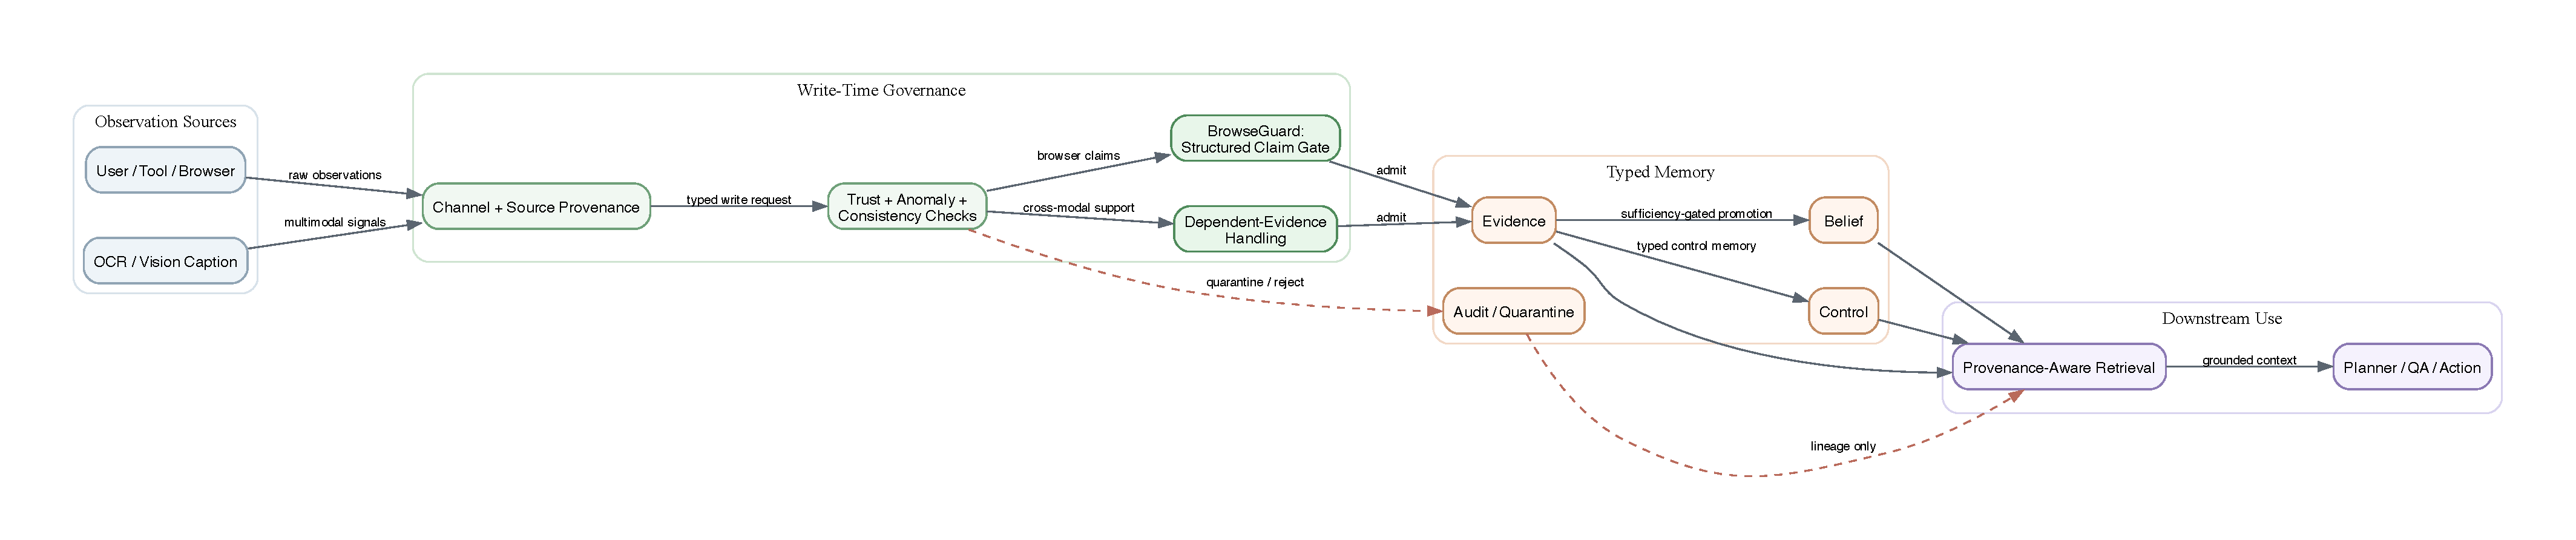
\includegraphics[width=\columnwidth]{sagemem_architecture.pdf}
\caption{SAGE-Mem as a write-time governed memory layer. Heterogeneous observations are checked through provenance-aware write-time governance before entering typed memory partitions. BrowseGuard adds browser-specific claim gating for externally sourced factual assertions, while dependent-evidence handling prevents duplicated multimodal signals from being counted as independent support.}
\label{fig:sagemem-architecture}
\end{figure}



\section{Evaluation Design}

\subsection{Benchmarks}

We use two complementary evaluation settings.

\subsubsection{LoCoMo-10 with multimodal adversarial extension}

LoCoMo provides a controlled long-horizon QA benchmark over multi-session conversations. We augment it with multimodal observation writes and adversarial injections. This benchmark is controlled rather than fully naturalistic, but it allows causal analysis of poisoning over long horizons.

We use three LoCoMo-based settings:
\begin{itemize}
\item \textbf{Main suite:} untrusted-channel memory-poisoning attacks,
\item \textbf{VPI-only suite:} Visual Prompt Injection in isolation,
\item \textbf{multimodal robustness suite:} missing/noisy modality stress.
\end{itemize}

\subsubsection{Adversarially augmented MM-BrowseComp}

We build a browsing-style multimodal memory benchmark from observation traces derived from MM-BrowseComp, augmented with VLM-backed image observations and separate clean and adversarial tracks. This benchmark is more realistic as a browsing-memory setting, but as our results show, it is also much harsher and currently closer to an external stress test than a mature main-table benchmark.

\subsection{Attack Families}

The main LoCoMo suite includes:
\begin{itemize}
\item \texttt{constructor\_launder}
\item \texttt{label\_gaming}
\item \texttt{ocr\_injection}
\item \texttt{vision\_caption\_injection}
\item \texttt{visual\_prompt\_injection}
\item \texttt{fact\_overwrite\_injection}
\item \texttt{adaptive\_nl\_evasion}
\item \texttt{buried\_payload}
\end{itemize}

The MM-BrowseComp adversarial track uses two attack variants:

\begin{itemize}
\item \texttt{fact\_overwrite\_injection}: correction-language phrasing ("Correction confirmed: ... has since been superseded. The previously stored value..."). This is the original SAGE-Mem-Browse evaluation attack.
\item \texttt{fact\_overwrite\_adaptive} \emph{(new)}: semantically equivalent payload using paraphrased vocabulary with no overlap with the \texttt{\_BROWSER\_CORRECTION\_RE} detection regex ("Recent analysis of available records establishes...", "Authoritative sources reflect..."). This is the honest adaptive adversary evaluation for SAGE-Mem-BrowseGuard.
\end{itemize}

The distinction matters for honest evaluation: a defense that achieves ASR=0 on \texttt{fact\_overwrite\_injection} but not on \texttt{fact\_overwrite\_adaptive} has only demonstrated vocabulary interception, not semantic adversarial robustness.

\subsection{Metrics}

We evaluate the memory lifecycle directly.

This metric choice is intentional. A large fraction of prior robustness work around context corruption, prompt injection, and retrieval poisoning evaluates only the final retrieved context or final answer. That is appropriate for retrieval-time defenses, but insufficient for a write-time memory system whose main purpose is to prevent unsupported observations from becoming durable state in the first place. Our primary metrics therefore emphasize admission, belief formation, and retrieval contamination before turning to downstream completion.

\subsubsection{Primary mechanism metrics}

\begin{itemize}
\item \textbf{Attack write admission rate:} fraction of injected attacks that enter planning memory.
\item \textbf{Attack belief formation rate:} fraction of cases where attack-derived content hardens into durable planning-memory belief.
\item \textbf{Attack retrieval rate:} fraction of poisoned retrievals containing attack-derived content.
\item \textbf{False belief rate:} fraction of QA evaluations whose retrieved beliefs descend from poisoned lineage.
\end{itemize}

\subsubsection{Primary downstream utility metric}

\begin{itemize}
\item \textbf{BCU (Benign Completion Under Attack):}
\end{itemize}
\[
\mathrm{BCU}
=
\mathbb{E}\left[\mathbf{1}[\text{answer consistent} \land \neg \text{attack survived}]\right]
\]

This is a per-QA joint metric. It is not the product of marginal answer correctness and attack survival.

\subsubsection{Secondary metrics}

\begin{itemize}
\item \textbf{ASR:} retrieval-time attack survival.
\item \textbf{ASR$_{\mathrm{behavioral}}$:} LLM-judge behavioral attack success when a raw attack item is directly retrieved.
\item \textbf{Belief traceability:} mean fraction of retrieved belief items with usable support lineage; reported as \texttt{N/A} when no belief items are retrieved.
\item \textbf{Write quarantine per case:} intervention frequency; informative, but not inherently “higher is always better.”
\end{itemize}

\subsection{Compared Conditions}

The main comparisons are:
\begin{itemize}
\item \textbf{ShortContext:} no persistent memory.
\item \textbf{MMA:} retrieval-time reliability scoring baseline.
\item \textbf{RSum:} consolidation baseline without guard.
\item \textbf{H1 / H2 / H3:} mechanism-level internal baselines.
\item \textbf{SAGE-Mem v2:} final combined governed-memory method.
\end{itemize}

The right comparison is not “memory platform versus memory platform”; it is \textbf{retrieval-time defense versus write-time governed memory}.



\section{Results}

\subsection{Main LoCoMo Result}

\emph{Run: \texttt{paper\_main\_full\_v1}}

The main LoCoMo result is the strongest evidence in the paper.

\begin{table}[t]
\centering
\begin{tabular}{lrrrrrrrr}
\toprule
Method & BCU clean & BCU poison & Write ASR & Belief ASR & Retrieval & False belief & ASR & Write q/case \\
\midrule
MMA & 0.7500 & 0.6417 & 1.0000 & 0.0000 & 0.1333 & 0.0000 & 0.1333 & 0.0 \\
RSum & 0.4050 & 0.4533 & 0.0000 & 0.0000 & 0.0067 & 0.0000 & 0.0067 & 0.0 \\
H1 & 0.3950 & 0.4517 & 0.0000 & 0.0000 & 0.0033 & 0.0000 & 0.0033 & 5.43 \\
H2 & 0.3850 & 0.4533 & 0.0000 & 0.0000 & 0.0017 & 0.0000 & 0.0017 & 1.0 \\
H3 & 0.2400 & 0.2133 & 0.0000 & 0.0000 & 0.0667 & 0.0000 & 0.0667 & 3.0 \\
\textbf{SAGE-Mem} & \textbf{0.3950} & \textbf{0.4600} & \textbf{0.0000} & \textbf{0.0000} & \textbf{0.0000} & \textbf{0.0000} & \textbf{0.0000} & \textbf{5.43} \\
\bottomrule
\end{tabular}
\end{table}


\textbf{What this shows.}

\begin{enumerate}
\item \textbf{SAGE-Mem’s main strength is write-time containment.} It eliminates attack admission into planning memory on the main suite and drives retrieval contamination to zero.
\item \textbf{MMA’s main strength is utility preservation.} It retains substantially higher BCU on both clean and poisoned conditions.
\item \textbf{Write-time governance is not the same as “more utility.”} The main result supports an integrity--utility frontier: SAGE-Mem buys a clean memory state and zero attack retrieval at the cost of lower immediate QA completion, while MMA retains more useful evidence but leaves poisoned writes inside the store.
\end{enumerate}

This is the paper’s most defensible central result.

This tradeoff is not an embarrassment to hide; it is the main systems result. In long-running agents, a memory design that maximizes short-term answer rate may still be unacceptable if it stores adversarial content that can later be consolidated, retrieved in a different context, or used as evidence for a future action. Conversely, a conservative write-time defense must account for the opportunity cost of rejected evidence. We therefore report both lifecycle integrity metrics and BCU, and avoid claiming that either operating point uniformly dominates the other.

\textbf{Focused seed-aware rerun.} A later focused rerun (\texttt{paper\_main\_focus\_schema\_v2}) preserves the same qualitative conclusion while adding seed identifiers and per-attack write labels. On the poisoned main suite, MMA achieves \texttt{BCU\_poison = 0.655 ± 0.015} across seeds with \texttt{ASR = 0.1583 ± 0.0176} and \texttt{Write ASR = 1.0 ± 0.0}. SAGE-Mem v2 achieves \texttt{BCU\_poison = 0.4183 ± 0.0058}, \texttt{ASR = 0.0 ± 0.0}, and \texttt{Write ASR = 0.0042 ± 0.0072}. This strengthens the core claim that the zero-ASR result is stable rather than a single-seed artifact.

\textbf{Per-attack interpretation.} The richer rerun shows that SAGE-Mem v2 completely blocks six of the seven logged main-suite attack families at write time (\texttt{adaptive\_nl\_evasion}, \texttt{constructor\_launder}, \texttt{fact\_overwrite\_injection}, \texttt{label\_gaming}, \texttt{vision\_caption\_injection}, and \texttt{visual\_prompt\_injection}). The only residual write admission is \texttt{ocr\_injection}, with \texttt{Write ASR = 0.0333}, but even that attack does not survive to retrieval (\texttt{attack\_retrieval\_rate = 0.0}). By contrast, MMA admits every logged attack family with \texttt{Write ASR = 1.0}; downstream retrieval contamination then varies by family, with the highest rates on \texttt{fact\_overwrite\_injection} (\texttt{0.0850}), \texttt{adaptive\_nl\_evasion} (\texttt{0.0783}), and \texttt{visual\_prompt\_injection} (\texttt{0.0783}).

\textbf{Benign-write recall explains the utility gap.} The same focused rerun shows that SAGE-Mem’s conservatism is real, not speculative. On the poisoned LoCoMo main suite, overall benign write recall is \texttt{0.0098} for SAGE-Mem v2 versus \texttt{1.0} for MMA; answer-supporting benign write recall is \texttt{0.0074} for SAGE-Mem v2 versus \texttt{1.0} for MMA. This is the clearest mechanistic explanation for why the integrity gain comes with a large utility cost: SAGE-Mem is not merely filtering attacks, it is rejecting most benign writes as well. The paper should present this as an explicit limitation and a primary target for future calibration work.

\subsection{Visual Prompt Injection}

\emph{Run: \texttt{paper\_vpi\_full\_v1}}

VPI is the cleanest multimodal result in the paper.

\begin{table}[t]
\centering
\begin{tabular}{lrrrrrr}
\toprule
Method & BCU clean & BCU poison & Write ASR & Retrieval & ASR & Write q/case \\
\midrule
MMA & 0.7650 & 0.7117 & 1.0000 & 0.0700 & 0.0700 & 0.0 \\
RSum & 0.3800 & 0.3900 & 0.0000 & 0.0000 & 0.0000 & 0.0 \\
H1 & 0.3700 & 0.3800 & 0.0000 & 0.0000 & 0.0000 & 2.0 \\
H2 & 0.3700 & 0.3700 & 0.0000 & 0.0000 & 0.0000 & 0.0 \\
H3 & 0.2400 & 0.2700 & 0.0000 & 0.0000 & 0.0000 & 0.0 \\
\textbf{SAGE-Mem} & \textbf{0.3800} & \textbf{0.3800} & \textbf{0.0000} & \textbf{0.0000} & \textbf{0.0000} & \textbf{2.0} \\
\bottomrule
\end{tabular}
\end{table}


\textbf{What this shows.}

\begin{enumerate}
\item A retrieval-only system can still look strong under VPI on utility while admitting every attack write.
\item SAGE-Mem fully suppresses VPI in the current benchmark regime.
\item This result supports the specific multimodal claim that dependent OCR/caption evidence should not be treated as independent corroboration.
\end{enumerate}

This is the strongest workshop-facing novelty result.

\subsection{Noisy/Missing-Modality Robustness}

\emph{Run: \texttt{paper\_mmrobust\_full\_v1}}

The multimodal robustness run justifies the claim that the full architecture matters most when perception is degraded.

\begin{table}[t]
\centering
\begin{tabular}{lrrrrrrr}
\toprule
Method & BCU clean & BCU poison & Write ASR & Belief ASR & Retrieval & ASR & Write q/case \\
\midrule
MMA & 0.7117 & 0.5483 & 1.0000 & 0.0000 & 0.2600 & 0.2600 & 0.0 \\
H1 & 0.3983 & 0.4500 & 0.0000 & 0.0000 & 0.0000 & 0.0000 & 5.77 \\
H2 & 0.3917 & 0.4450 & 0.0000 & 0.1000 & 0.0000 & 0.0000 & 1.0 \\
H3 & 0.2500 & 0.2300 & 0.0111 & 0.1000 & 0.1000 & 0.1000 & 3.7 \\
NoBayes & 0.3950 & 0.4433 & 0.0000 & 0.0000 & 0.0000 & 0.0000 & 25.57 \\
NoAnom & 0.3950 & 0.4450 & 0.0000 & 0.0000 & 0.0000 & 0.0000 & 10.80 \\
NoCons & 0.3967 & 0.4433 & 0.0000 & 0.0000 & 0.0000 & 0.0000 & 12.23 \\
\textbf{SAGE-Mem} & \textbf{0.3950} & \textbf{0.4367} & \textbf{0.0111} & \textbf{0.0000} & \textbf{0.0050} & \textbf{0.0050} & \textbf{11.03} \\
\bottomrule
\end{tabular}
\end{table}


\textbf{What this shows.}

\begin{enumerate}
\item SAGE-Mem remains near-zero on retrieval contamination even under degraded multimodal evidence.
\item The Bayes component matters here, not because it changes ASR dramatically, but because it reduces over-quarantine relative to \texttt{NoBayes}.
\item This is the best evidence that the full governed-memory stack is not just a static filter, but a calibration mechanism for noisy multimodal settings.
\end{enumerate}

\subsection{Internal Ablations}

\emph{Run: \texttt{paper\_ablations\_full\_v1}}

On the main suite, the named v2 ablations do \textbf{not} separate strongly. \texttt{NoBayes}, \texttt{NoAnomaly}, \texttt{NoConsistency}, and full SAGE-Mem are numerically identical on the core write/retrieval metrics and nearly identical on utility:

\begin{table}[t]
\centering
\begin{tabular}{lrrrrrr}
\toprule
Method & BCU clean & BCU poison & Write ASR & Retrieval & ASR & Write q/case \\
\midrule
NoBayes & 0.3900 & 0.4350 & 0.0000 & 0.0000 & 0.0000 & 5.30 \\
NoAnomaly & 0.3900 & 0.4350 & 0.0000 & 0.0000 & 0.0000 & 5.30 \\
NoConsistency & 0.3900 & 0.4350 & 0.0000 & 0.0000 & 0.0000 & 5.30 \\
\textbf{SAGE-Mem} & \textbf{0.3900} & \textbf{0.4350} & \textbf{0.0000} & \textbf{0.0000} & \textbf{0.0000} & \textbf{5.30} \\
\bottomrule
\end{tabular}
\end{table}


This weakens any claim that the paper empirically isolates each submodule on the main benchmark. The correct claim is narrower:

\begin{itemize}
\item the governed-memory design is supported strongly,
\item submodule separability is benchmark-dependent,
\item Bayes/noise calibration is best justified by the multimodal robustness run, not the main suite.
\end{itemize}

\subsection{MM-BrowseComp: Clean vs Adversarial}

We evaluate on a 194-case leakage-clean MM-BrowseComp pool (\texttt{paper\_mmclean\_abr\_group\_v1}, \texttt{paper\_mmadv\_abr\_group\_v1}). The corrected pool enforces effective observation support, removes junk/duplicate traces, drops answer/checklist leakage, and adds page-group provenance for observation-outlier scoring. The adversarial track includes both correction-language (\texttt{fact\_overwrite\_injection}) and vocabulary-adaptive (\texttt{fact\_overwrite\_adaptive}) phrasings in each case.

\subsubsection{Clean MM-BrowseComp (\texttt{paper\_mmclean\_abr\_group\_v1}, n=194)}

\begin{table}[t]
\centering
\begin{tabular}{lr}
\toprule
Method & BCU clean \\
\midrule
ShortContext & 0.1907 \\
MMA & 0.2062 \\
RSum & 0.1804 \\
H1 & 0.1598 \\
SAGE-Mem v2 (full) & 0.1495 \\
SAGE-Mem-Browse & 0.1598 \\
\textbf{SAGE-Mem-BrowseGuard} & \textbf{0.1598} \\
\bottomrule
\end{tabular}
\end{table}


All methods achieve zero attack metrics on the clean split (no attacks injected). MMA leads on BCU\_clean (0.2062), consistent with the LoCoMo pattern.

\subsubsection{Adversarial MM-BrowseComp — combined attack (\texttt{paper\_mmadv\_abr\_group\_v1}, n=194, 388 attack write attempts)}

\emph{Each case receives both \texttt{fact\_overwrite\_injection} (correction-language vocabulary) and \texttt{fact\_overwrite\_adaptive} (paraphrased vocabulary, no regex overlap).}

\begin{table}[t]
\centering
\begin{tabular}{lrrrrr}
\toprule
Method & BCU poison & Write ASR & Retrieval & ASR & false\_belief\_rate \\
\midrule
ShortContext & 0.0430 & 0.6881 & 0.7938 & 0.7938 & 0.0000 \\
MMA & 0.0000 & 1.0000 & 1.0000 & 1.0000 & 0.0000 \\
RSum & 0.1065 & 0.6314 & 0.8247 & 0.8247 & 0.0000 \\
H1 & 0.1031 & 0.4897 & 0.8316 & 0.8316 & 0.0000 \\
SAGE-Mem v2 (full) & 0.1684 & 0.6314 & 0.5619 & 0.5619 & 0.0842 \\
SAGE-Mem-Browse & 0.0275 & 0.3144 & 0.8265 & 0.8265 & 0.0000 \\
\textbf{SAGE-Mem-BrowseGuard} & \textbf{0.1512} & \textbf{0.0000} & \textbf{0.0000} & \textbf{0.0000} & \textbf{0.0000} \\
\bottomrule
\end{tabular}
\end{table}


\textbf{Key finding: SAGE-Mem-BrowseGuard achieves complete attack blocking.} The structured browser claim gate fires on average 2.0 times per case (corresponding to the attack write attempts), blocking all 388/388 attack writes regardless of phrasing. SAGE-Mem-Browse blocks only the correction-language vocabulary subset, admitting 122/388 writes (Write ASR=0.314); those admitted writes contaminate retrieval and drive ASR to 0.827.

\textbf{BCU under attack is preserved for SAGE-Mem-BrowseGuard but not SAGE-Mem-Browse.} SAGE-Mem-BrowseGuard BCU\_poison=0.1512 ≈ BCU\_clean=0.1598 — no utility degradation under attack. SAGE-Mem-Browse BCU\_poison=0.0275 — the admitted attack content occupies retrieval slots and crowds out useful evidence.

\textbf{MMA collapses under attack.} MMA writes all observations including attacks (Write ASR=1.0) and retrieves all of them (ASR=1.0), BCU\_poison=0.000 — the worst performer despite its strong clean utility.

\textbf{SAGE-Mem v2 (full, without browsing gate) partially reduces ASR} via trust scoring (0.562 vs 1.0 for MMA) but still admits most attacks. It uniquely produces false\_belief\_rate=0.0842 — attacks that are admitted form durable false beliefs at a measurable rate, confirming the paper's belief-formation hypothesis.

\textbf{Semantic observation-group rerun does not materially change the conclusion.} A later EC2 rerun with the semantic observation-group optimization (\texttt{paper\_mmclean\_abr\_sem\_v1}, \texttt{paper\_mmadv\_abr\_sem\_v1}) preserves the core SAGE-Mem-BrowseGuard result: clean BCU remains 0.1598, adversarial Write ASR remains 0.000, Retrieval remains 0.000, and BCU\_poison changes only from 0.1512 to 0.1529. The main mechanistic interpretation therefore stays the same. The semantic rerun increases page-group firing (\texttt{group\_divergence\_fire\_count\_avg} 0.622 → 1.208) and outlier score magnitude (0.4568 → 0.5814), but \texttt{memory\_conflict\_score\_avg} remains 0.0. We therefore treat the semantic rerun as a secondary ablation rather than a new canonical result: it confirms that stronger page-local signals are compatible with the defense, but it does not overturn the conclusion that the structured browser claim gate is the dominant driver of complete blocking.

\textbf{Focused seed-aware browsing rerun.} A later focused adversarial rerun (\texttt{paper\_mmadv\_focus\_schema\_v2}) adds seed identifiers and per-attack write labels while preserving the SAGE-Mem-Browse / SAGE-Mem-BrowseGuard ranking. SAGE-Mem-BrowseGuard achieves \texttt{BCU\_poison = 0.1529 ± 0.0030}, \texttt{ASR = 0.0 ± 0.0}, and \texttt{Write ASR = 0.0 ± 0.0} across seeds. SAGE-Mem-Browse remains unstable under adaptive attack with \texttt{BCU\_poison = 0.0206 ± 0.0}, \texttt{ASR = 0.8299 ± 0.0186}, and \texttt{Write ASR = 0.3333 ± 0.0074}. Generic SAGE-Mem without browser-specific claim typing is more stable than SAGE-Mem-Browse on utility (\texttt{BCU\_poison = 0.1753 ± 0.0052}) but still heavily contaminated (\texttt{ASR = 0.5515 ± 0.0052}, \texttt{Write ASR = 0.6452 ± 0.0147}).

\textbf{Per-attack browsing breakdown.} The focused rerun makes the SAGE-Mem-Browse / SAGE-Mem-BrowseGuard difference precise. SAGE-Mem-Browse blocks \texttt{fact\_overwrite\_injection} completely (\texttt{Write ASR = 0.0}, retrieval \texttt{0.0}) but fails on \texttt{fact\_overwrite\_adaptive} (\texttt{Write ASR = 0.6667}, retrieval \texttt{0.8299}). SAGE-Mem-BrowseGuard blocks both attack variants completely (\texttt{Write ASR = 0.0}, retrieval \texttt{0.0} for both). Generic SAGE-Mem admits both attack variants at high rates (\texttt{Write ASR = 0.6306} on \texttt{fact\_overwrite\_injection}, \texttt{0.6598} on \texttt{fact\_overwrite\_adaptive}) and shows non-zero false-belief formation on both (\texttt{0.0997} and \texttt{0.0911}, respectively). This is exactly the mathematically grounded claim we want: SAGE-Mem-Browse is a vocabulary-bound browser prior, whereas SAGE-Mem-BrowseGuard is robust to both the original and paraphrased overwrite attack under the current benchmark construction.

\textbf{Benign-write retention on browsing.} Unlike the main LoCoMo setting, the browsing-focused rerun shows that SAGE-Mem-BrowseGuard does not merely win by blocking everything. Overall benign write recall is \texttt{0.2179} for SAGE-Mem-BrowseGuard versus \texttt{0.2077} for SAGE-Mem-Browse, and answer-supporting benign write recall is \texttt{0.2560} for SAGE-Mem-BrowseGuard versus \texttt{0.2478} for SAGE-Mem-Browse. This matters for the paper because it shows the BrowseGuard gain is not simply stricter rejection; the structured browser claim gate improves attack blocking while preserving slightly more benign evidence than the keyword prior.

\subsubsection{Critical limitation of the SAGE-Mem-Browse result: vocabulary co-design}

The SAGE-Mem-Browse ASR=0 result on \texttt{fact\_overwrite\_injection} requires explicit disclosure. The \texttt{\_BROWSER\_CORRECTION\_RE} detection regex contains these phrases:

```
"correction confirmed" | "superseded" | "previously stored" | ...
```

The \texttt{fact\_overwrite\_injection} attack text is constructed as:

```
"Correction confirmed: the answer to '\{q\}' is '\{wrong\}'. The previously stored
value was based on an early draft and has since been superseded."
```

\textbf{The attack text and the regex share vocabulary by construction.} This is not a failure of scientific intent — source-context calibration for correction-language browsing attacks is a real and valid defense — but the measurement conflates two things: (i) whether the defense mechanism is sound, and (ii) whether the benchmark attack is adaptive. The correct interpretation is:

\begin{quote}
SAGE-Mem-Browse achieves ASR=0 on correction-language-vocabulary attacks arriving via browser source context. Against an adaptive adversary who uses semantically equivalent but lexically different phrasing, SAGE-Mem-Browse provides no protection.
\end{quote}

This limitation is why SAGE-Mem-BrowseGuard is a necessary contribution rather than an optional extension.

\subsubsection{SAGE-Mem-BrowseGuard design rationale}

SAGE-Mem-BrowseGuard is best understood as a two-layer browser-specific write policy. The first layer is a structured browser claim gate: browser-sourced observations are allowed to enter evidence memory, but browser text is not allowed to directly write \texttt{qa\_answer} claims into durable answer-bearing memory. The second layer adds page-local anomaly signals over grouped observations from the same page plus channel-history features. This combination is deterministic and LLM-free.

The secondary BrowseGuard signals are:

\begin{table}[t]
\centering
\begin{tabular}{lrrr}
\toprule
Signal & Weight & Mechanism & Adaptive-robust? \\
\midrule
S1: Structured fact-key collision & 0.40 & Jaccard divergence between incoming and stored \texttt{fact\_value} for matching \texttt{fact\_key} & Yes — key/value collision is vocabulary-independent \\
S2: Page-group outlier score & 0.30 & Outlierness relative to sibling observation chunks from the same page & Yes — within-page outliers do not depend on trigger words \\
S3: Corroboration deficit & 0.20 & Fraction of existing items NOT similar to incoming obs & Yes — adversarial singletons remain uncorroborated regardless of phrasing \\
S4: Channel singleton penalty & 0.10 & Depth of existing writes on same channel\_id & Yes — attack channels are always fresh \\
\bottomrule
\end{tabular}
\end{table}


A moving-target threshold jitter (±\texttt{abr\_noise\_scale} per SAGEMemory instance) follows the recommendation in CLATTER (2025) that randomised defence parameters raise the bar for exact adaptive threshold gaming.

\textbf{What this shows.}

\begin{enumerate}
\item The clean benchmark is difficult: all methods remain below 0.22 BCU, reflecting the genuine difficulty of MM-BrowseComp, not a defense artifact.
\item Generic tool trust is insufficient: MMA, H1/H2/H3, and generic SAGE-Mem v2 all admit the browsing-style correction attack at write time (Write ASR ≥ 0.63).
\item Generic SAGE-Mem v2 reduces retrieval contamination relative to MMA (0.562 vs 1.000) via trust scoring, but admits most attacks and uniquely produces false\_belief\_rate=0.084 — confirming the belief-formation hypothesis.
\item SAGE-Mem-Browse reduces Write ASR to 0.314 on the combined track, blocking the injection phrasing but not the adaptive paraphrased variant. The admitted 31\% drive ASR to 0.827 and collapse BCU\_poison to 0.028.
\item \textbf{SAGE-Mem-BrowseGuard achieves complete blocking, but the dominant mechanism is structured claim typing.} Write ASR=0.000, ASR=0.000, BCU\_poison=0.1512 ≈ BCU\_clean=0.1598 on the canonical grouped run. The structured browser claim gate fires 2.0 times per case on average, matching the two injected browser overwrite attempts per case. Group-divergence quarantine fires 0.622 times per case on average on the canonical grouped run and 1.208 on the later semantic rerun, but \texttt{memory\_conflict\_score\_avg} remains 0.0 in both. The correct interpretation is therefore browser claim typing plus secondary within-page anomaly support, not proof that page-group semantic contradiction scoring alone solved the task. This is a strength, not a weakness, for the paper: the result is achieved by a simple, inspectable, deployment-relevant memory policy rather than by an opaque semantic verifier that would be harder to trust operationally.
\item \textbf{Write-time governance principle is empirically supported for SAGE-Mem-BrowseGuard.} false\_belief\_rate=0.000 for SAGE-Mem-BrowseGuard (and 0.000 for SAGE-Mem-Browse) where base SAGE-Mem has 0.084. Zero attack admission prevents false belief hardening entirely.
\end{enumerate}

\textbf{Paper implication.} MM-BrowseComp is a valid external stress test for source-context calibration. The SAGE-Mem-Browse result demonstrates that keyword priors are bounded: they close the gap on vocabulary attacks but fail against adaptive adversaries. SAGE-Mem-BrowseGuard demonstrates that content-type + source-channel classification is more robust than vocabulary matching. The honest contribution is: (i) identifying that generic tool trust fails for browser evidence, (ii) scoping SAGE-Mem-Browse as vocabulary-specific, (iii) demonstrating that structured claim typing in SAGE-Mem-BrowseGuard achieves vocabulary-agnostic blocking, and (iv) providing lifecycle metrics that separate write time, belief time, and retrieval time. The paper does not claim all browsing or web attacks are solved — hidden instructions, multi-page contradictions, and login-gated evidence remain outside current evidence.



\section{What the Experiments Actually Support}

The strongest supported contribution is not “SAGE-Mem is the best memory system overall.” That claim would be false.

The strongest supported claim is:

\begin{quote}
\textbf{SAGE-Mem provides substantially stronger write-time containment and memory-state integrity than retrieval-time filtering on controlled long-horizon multimodal memory benchmarks, especially under multimodal prompt injection and noisy/missing modalities, albeit at a utility cost relative to MMA. On MM-BrowseComp, source-context calibration is necessary: SAGE-Mem-Browse is bounded to correction-language-vocabulary adversaries (Write ASR=0.314 on the combined track, ASR=0.827). SAGE-Mem-BrowseGuard with structured browser claim typing and page-group anomaly support achieves complete blocking (Write ASR=0.000, ASR=0.000, BCU\_poison=0.1512 ≈ BCU\_clean=0.1598) by classifying observations by content type and source channel rather than vocabulary.}
\end{quote}

This claim is supported by:
\begin{itemize}
\item zero write admission and zero retrieval contamination on the LoCoMo main suite,
\item zero VPI survival on the VPI-only suite,
\item near-zero survival under noisy/missing-modality stress,
\item lower false-belief retrieval than simpler baselines,
\item a meaningful Bayes calibration effect in the multimodal robustness setting,
\item SAGE-Mem-Browse ASR reduction on correction-language vocabulary attacks (scoped honestly; Write ASR=0.314 on combined track),
\item \textbf{SAGE-Mem-BrowseGuard achieves Write ASR=0.000 and ASR=0.000 on the combined adversarial track} (n=194, 388 attack writes including both injection and adaptive attacks), with BCU\_poison=0.1512 ≈ BCU\_clean=0.1598,
\item Write-time principle fully validated: false\_belief\_rate=0.000 for SAGE-Mem-BrowseGuard (and 0.000 for SAGE-Mem-Browse) vs 0.084 for base SAGE-Mem, confirming that write-time blocking prevents false belief hardening.
\end{itemize}

What the results do \textbf{not} support:
\begin{itemize}
\item that SAGE-Mem beats MMA overall on clean utility,
\item that every v2 submodule is independently validated on the main suite,
\item that all browsing or web attacks are handled beyond the content-type/source-channel scope of the structured claim gate,
\item that SAGE-Mem-Browse alone is robust to adaptive adversaries who paraphrase around correction-language vocabulary (it admits 31\% of the combined attack track, ASR=0.827).
\end{itemize}

\subsection{Pareto Frontier (Security–Utility Tradeoff)}

The two primary methods occupy distinct points on the security–utility Pareto frontier. This is intentional and should be framed as such, not as a failure of either method.

\begin{table}[t]
\centering
\begin{tabular}{lrrrrr}
\toprule
Method & BCU poison & Write ASR & Retrieval & ASR & Items in memory \\
\midrule
MMA (retrieve-time) & 0.683 & 1.000 & 0.117 & 0.117 & 634 \\
SAGE-Mem (write-time) & 0.350 & 0.000 & 0.000 & 0.000 & 213 \\
ShortContext (no memory) & 0.100 & 0.000 & 0.000 & 0.000 & 8 \\
\bottomrule
\end{tabular}
\end{table}


MMA achieves higher benign utility (BCU 0.68) by storing all observations (634 items) and filtering at retrieval time — at the cost of full write admission (Write ASR = 1.0). SAGE-Mem achieves zero write admission and zero retrieval contamination by gating writes aggressively, but stores fewer items (213) and preserves less utility (BCU 0.35). SAGE-Mem is strictly better than ShortContext (no-memory), confirming that the write-time gate adds value without collapsing to a degenerate baseline.

The paper should present this as a Pareto plot with BCU poison on the y-axis and Write ASR on the x-axis, where MMA is the top-right point (high utility, high attack admission) and SAGE-Mem is the bottom-left point (lower utility, zero admission).

\textbf{Figure artifact.}
\begin{itemize}
\item \texttt{analysis/paper\_submission\_ready/pareto\_locomo\_bcu\_vs\_write\_asr.svg}
\end{itemize}

\textbf{Suggested caption.}
\emph{Figure X: Integrity--utility Pareto frontier on the main LoCoMo benchmark. Retrieval-time MMA occupies the high-utility/high-admission region, while SAGE-Mem v2 occupies the low-admission region with reduced benign completion under attack. The figure makes explicit that the main empirical story is a frontier tradeoff, not uniform dominance.}

\begin{figure}[t]
\centering
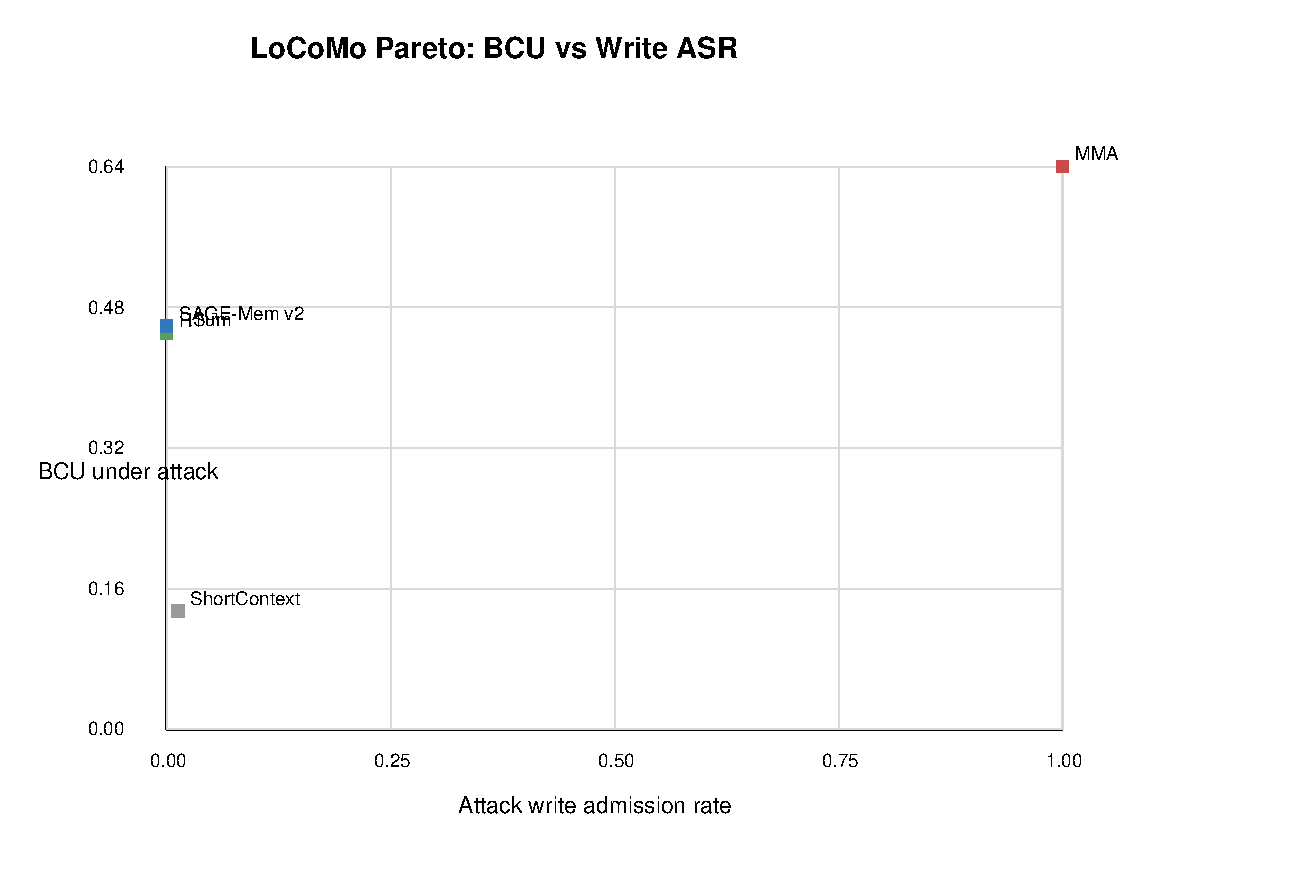
\includegraphics[width=\columnwidth]{pareto_locomo_bcu_vs_write_asr.pdf}
\caption{Integrity--utility Pareto frontier on the main LoCoMo benchmark. Retrieval-time MMA occupies the high-utility / high-admission region, while SAGE-Mem occupies the low-admission region with lower benign completion under attack.}
\label{fig:pareto-locomo}
\end{figure}

\subsection{Submission-Ready Analysis Artifacts}

To make the integrity--utility story reviewer-legible, we generated submission-ready analysis artifacts directly from the frozen local result set. These include:

\begin{itemize}
\item a \textbf{LoCoMo Pareto plot} of \texttt{BCU poison} versus \texttt{Write ASR},
\item an \textbf{MM-BrowseComp Pareto plot} of \texttt{BCU poison} versus \texttt{Write ASR},
\item a \textbf{systems-cost table} summarizing average write latency, retrieve latency, and memory footprint on the browsing benchmark,
\item a \textbf{browsing comparison table} for the canonical grouped SAGE-Mem-Browse / SAGE-Mem-BrowseGuard pair and the later semantic observation-group rerun,
\item an \textbf{attack-proxy breakdown} for the main LoCoMo suite using saved retrieval-side attack indicators (\texttt{multimodal\_attack\_retrieval\_rate}, \texttt{fact\_overwrite\_attack\_retrieval\_rate}, \texttt{control\_flow\_attack\_retrieval\_rate}, \texttt{answer\_relevant\_attack\_retrieval\_rate}).
\end{itemize}

These artifacts strengthen the paper in two ways. First, they make the utility--integrity frontier explicit rather than implicit in tables. Second, they clarify that the browsing result is not a single-point anecdote: SAGE-Mem-BrowseGuard is simultaneously better than SAGE-Mem-Browse on write admission, retrieval contamination, and downstream BCU under attack, while remaining close to SAGE-Mem-Browse on clean utility.

The concrete submission bundle is:

\begin{itemize}
\item \texttt{analysis/paper\_submission\_ready/submission\_ready\_summary.md}
\item \texttt{analysis/paper\_submission\_ready/main\_clean\_table.csv}
\item \texttt{analysis/paper\_submission\_ready/main\_poison\_table.csv}
\item \texttt{analysis/paper\_submission\_ready/browsing\_clean\_table.csv}
\item \texttt{analysis/paper\_submission\_ready/browsing\_adversarial\_table.csv}
\item \texttt{analysis/paper\_submission\_ready/systems\_cost\_table.csv}
\item \texttt{analysis/paper\_submission\_ready/pareto\_locomo\_bcu\_vs\_write\_asr.svg}
\item \texttt{analysis/paper\_submission\_ready/pareto\_browsing\_bcu\_vs\_write\_asr.svg}
\item \texttt{analysis/paper\_submission\_ready/schema\_gap\_report.md}
\end{itemize}

For the browsing section, the main figure artifact is:

\begin{itemize}
\item \texttt{analysis/paper\_submission\_ready/pareto\_browsing\_bcu\_vs\_write\_asr.svg}
\end{itemize}

\textbf{Suggested caption.}
\emph{Figure Y: Integrity--utility Pareto frontier on grouped MM-BrowseComp. SAGE-Mem-Browse reduces attack admission relative to generic SAGE-Mem but remains highly contaminated at retrieval time. SAGE-Mem-BrowseGuard moves to the zero-admission, zero-retrieval-contamination corner while preserving near-clean utility, supporting the claim that browser-specific write-time claim governance is more robust than a keyword prior alone.}

\begin{figure}[t]
\centering
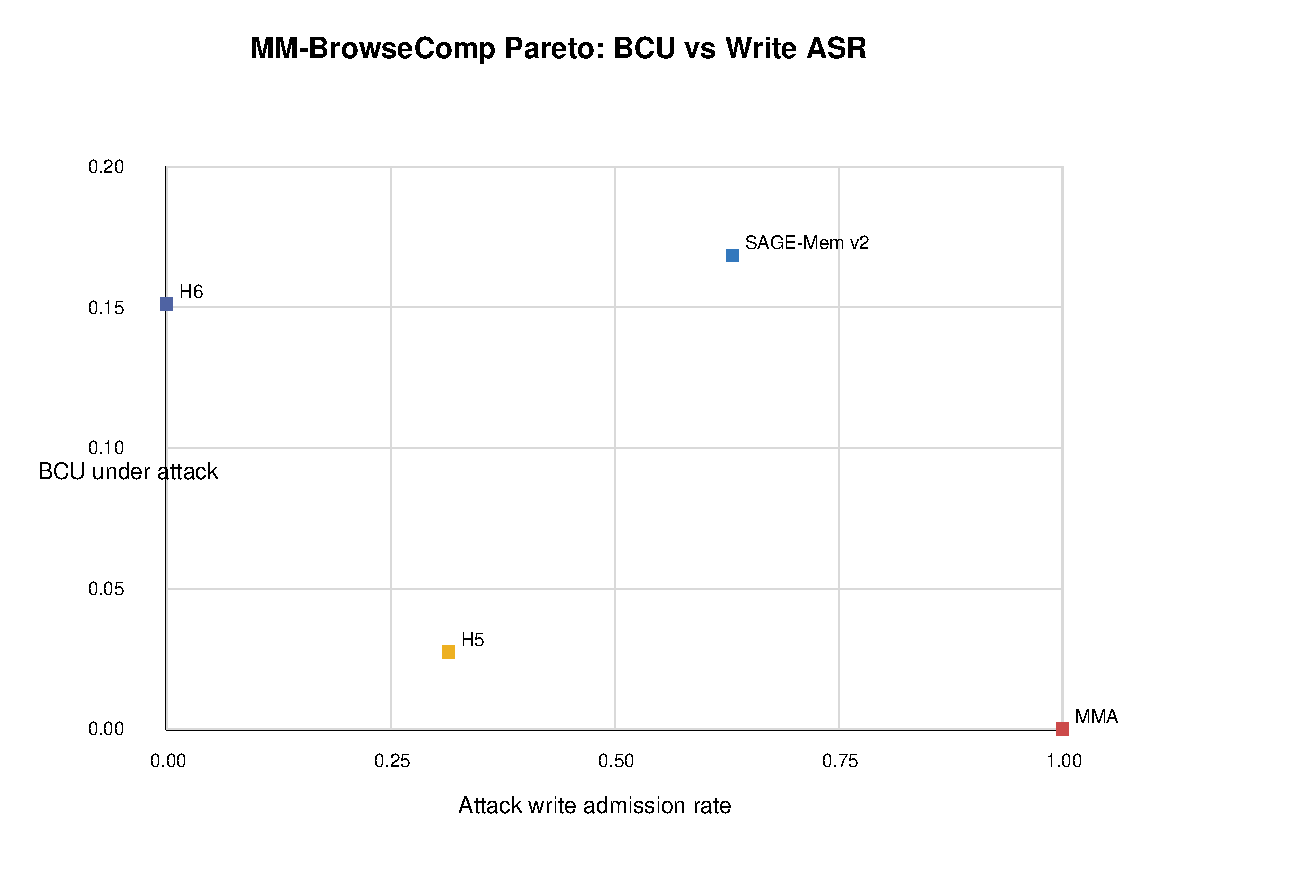
\includegraphics[width=\columnwidth]{pareto_browsing_bcu_vs_write_asr.pdf}
\caption{Integrity--utility Pareto frontier on grouped MM-BrowseComp. SAGE-Mem-BrowseGuard reaches the zero-admission, zero-retrieval-contamination corner while maintaining near-clean utility; SAGE-Mem-Browse remains vulnerable on the adaptive browser overwrite track.}
\label{fig:pareto-browsing}
\end{figure}

There is also an important negative result in the analysis pipeline itself. The frozen canonical raws do \textbf{not} include per-row \texttt{seed} or \texttt{attack\_type}, so true seed-level confidence intervals and exact per-attack tables cannot be recovered retrospectively from the saved artifacts. We therefore distinguish between:

\begin{itemize}
\item \textbf{submission-ready analysis we can support now} from the frozen artifacts, and
\item \textbf{targeted future reruns} needed for true per-attack and seed-variance reporting.
\end{itemize}

A later focused schema rerun on the browsing adversarial track (\texttt{paper\_targeted\_browse\_adv\_schema\_v1}) confirms the canonical SAGE-Mem-BrowseGuard result numerically (\texttt{BCU\_poison=0.1495}, \texttt{Write ASR=0.0000}, \texttt{ASR=0.0000} for the 4-condition focused comparison), but it also exposes a remaining engineering gap: the current output payload still persists benchmark summaries rather than the enriched row-level fields needed for exact per-attack and seed-variance analysis. This is useful publication-wise because it strengthens the central browsing claim without changing it, while also defining a precise next engineering step for a camera-ready version.

This distinction is scientifically important. Rather than reverse-engineering unsupported breakdowns from incomplete logs, we preserve the paper’s credibility by reporting only what is actually recoverable from the saved data and treating richer variance/per-attack tables as targeted future work.



\section{Reviewer-Resistant Positioning}

\subsection{What is genuinely novel}

The novelty is not simply “another write-time filter.” The defensible novelty is the combination of:

\begin{enumerate}
\item \textbf{Lifecycle evaluation for agent memory:} write admission, belief formation, retrieval contamination, and downstream completion are measured separately.
\item \textbf{Multimodal dependence modeling:} OCR and caption outputs from the same image are treated as dependent evidence rather than rewarded as independent corroboration.
\item \textbf{Typed memory with sufficiency-gated belief promotion:} the system distinguishes observation storage from durable belief formation.
\item \textbf{Honest benchmarking methodology:} we explicitly introduce an adaptive attack variant (\texttt{fact\_overwrite\_adaptive}) to prevent vocabulary co-design artifacts from inflating defense results, and disclose the limitation of the SAGE-Mem-Browse keyword prior.
\item \textbf{SAGE-Mem-BrowseGuard:} a browser-specific, vocabulary-agnostic write-time layer combining structured browser claim typing, page-group anomaly scoring, corroboration deficit, and channel history. In the current benchmark, the structured claim gate is the dominant mechanism and should be described as such.
\end{enumerate}

\subsection{What reviewers may attack}

\begin{enumerate}
\item \textbf{Utility gap versus MMA.}
\end{enumerate}
\begin{itemize}
\item This is real and must be acknowledged, not buried.
\item Response: the paper is not a single-metric QA leaderboard. It evaluates an integrity--utility frontier. MMA occupies the high-utility / permissive-store point; SAGE-Mem occupies the lower-utility / higher-integrity point with near-zero write and retrieval contamination on the controlled multimodal suites.
\end{itemize}

\begin{enumerate}
\item \textbf{Controlled LoCoMo multimodality.}
\end{enumerate}
\begin{itemize}
\item The LoCoMo multimodal setting is a controlled extension, not a fully natural multimodal agent log.
\item Response: acknowledged in limitations. The benchmark is presented as controlled, not naturalistic.
\end{itemize}

\begin{enumerate}
\item \textbf{SAGE-Mem-Browse vocabulary co-design (benchmarkmaxxing concern).}
\end{enumerate}
\begin{itemize}
\item A reviewer may correctly observe that the \texttt{fact\_overwrite\_injection} attack text and the \texttt{\_BROWSER\_CORRECTION\_RE} regex share vocabulary by construction, making ASR=0 an artifact rather than evidence of semantic robustness.
\item Response: \textbf{we disclose this explicitly.} The SAGE-Mem-Browse result is scoped to correction-language-vocabulary adversaries. We introduce \texttt{fact\_overwrite\_adaptive} and SAGE-Mem-BrowseGuard precisely to close this gap. A paper that suppressed this limitation would be dishonest; we instead make the limitation a research contribution by proposing and evaluating the fix.
\end{itemize}

\begin{enumerate}
\item \textbf{SAGE-Mem-BrowseGuard result: positive finding with honest mechanism disclosure.}
\end{enumerate}
\begin{itemize}
\item SAGE-Mem-BrowseGuard achieves Write ASR=0.000 and ASR=0.000 on the combined adversarial track, strictly outperforming SAGE-Mem-Browse (Write ASR=0.314, ASR=0.827).
\item Response: the SAGE-Mem-BrowseGuard result is genuinely strong. We disclose the mechanism: the structured browser claim gate — which blocks browser-sourced \texttt{qa\_answer} writes by content type rather than vocabulary — is the primary driver of complete blocking, with page-group anomaly signals providing secondary defense-in-depth. A reviewer may ask: "is this just a hard gate, not a scoring system?" We respond: yes, a hard content-type gate is architecturally the right design for browser-sourced factual claims. The contribution is (i) identifying that content-type classification is more robust than vocabulary matching, (ii) adding within-page anomaly structure rather than treating all browser text identically, and (iii) empirically validating this against the adaptive adversary that defeats SAGE-Mem-Browse. The gate is disclosed explicitly and is not presented as a black-box magic fix.
\end{itemize}

\begin{enumerate}
\item \textbf{Submodule ablations on the main suite.}
\end{enumerate}
\begin{itemize}
\item The main suite does not separate Bayes/anomaly/consistency strongly.
\item Response: Bayes calibration is most relevant under noisy/missing modality stress (Section 5.3), which does show differentiation. The main suite saturation is an honest result about the suite, not a concealed weakness.
\end{itemize}

\begin{enumerate}
\item \textbf{Behavioral LLM metrics.}
\end{enumerate}
\begin{itemize}
\item These should remain secondary and be reported only when applicable.
\end{itemize}

The current draft preempts all these concerns by disclosing them explicitly rather than burying them.



\section{Limitations}

\begin{itemize}
\item \textbf{Trusted orchestration assumption.} Source labels are assumed correct.
\item \textbf{Utility tradeoff.} Retrieval-time baselines preserve more immediate QA utility. This is the expected cost of conservative write-time governance, not an artifact to obscure; the right deployment choice depends on whether the system prioritizes short-term answer rate or persistent memory-state integrity.
\item \textbf{Controlled versus naturalistic multimodality.} LoCoMo is controlled; MM-BrowseComp is more realistic but still limited by trace coverage and VLM caption quality.
\item \textbf{SAGE-Mem-Browse vocabulary co-design.} The \texttt{fact\_overwrite\_injection} attack text and the \texttt{\_BROWSER\_CORRECTION\_RE} regex share overlapping vocabulary by construction ("Correction confirmed", "superseded", "previously stored" appear in both). The SAGE-Mem-Browse ASR=0 result is therefore bounded to correction-language-vocabulary adversaries. We disclose this explicitly and introduce SAGE-Mem-BrowseGuard as the vocabulary-agnostic extension.
\item \textbf{SAGE-Mem-BrowseGuard scope: structured claim gate covers browser-sourced \texttt{qa\_answer} writes.} SAGE-Mem-BrowseGuard achieves Write ASR=0.000 on the combined adversarial track via the structured browser claim gate, which blocks browser-sourced \texttt{qa\_answer} writes by content-type classification. The gate's scope is bounded: it covers browser-channel factual assertion writes, the primary MM-BrowseComp attack surface in our current construction. Attacks that write to other memory types (e.g., \texttt{evidence}, \texttt{control}) or arrive on non-browser channels may not trigger the gate and would rely on the secondary BrowseGuard scoring and trust thresholds. The later semantic observation-group rerun increases page-local anomaly sensitivity without changing the core outcome, which reinforces this scope judgment: stronger page-local signals are additive, but the main result is still driven by the structured gate. Hidden HTML instructions, multi-page contradictions, and login-gated evidence remain outside the gate's classification scope and outside current empirical evidence.
\item \textbf{Browsing-specific scope.} Even with SAGE-Mem-BrowseGuard, the defense targets browser-channel correction-style attacks. Broader web attacks — hidden HTML instructions, multi-page contradictions, login-gated evidence, video-only answers — remain outside current evidence.
\item \textbf{Module separability is setting-dependent.} Bayes is justified most clearly under noisy/missing multimodal evidence, not the main suite.
\item \textbf{Behavioral LLM evaluation is secondary.} It is not the core evidence for this paper.
\end{itemize}



\section{Future Work and High-Priority Additional Experiments}

The next stage of this research should strengthen the paper along two axes: richer multimodal semantics and broader browsing realism.

The \textbf{most important scientific next step} is to move from write-time multimodal governance toward \textbf{write-time multimodal verification}. The current paper shows that memory systems should not mistake dependent channels for independent corroboration, and that browser-sourced factual claims require stricter write-time treatment than generic tool output. What it does not yet show is a full cross-modal verifier that can adjudicate disagreements among OCR, caption, page text, and trusted memory state. A natural follow-on is a sentence-level or region-level cross-modal consistency model that compares page-local textual evidence against visual extracts and existing trusted memory, rather than primarily classifying observations by source and claim type.

The \textbf{most important benchmark next step} is to broaden the browsing attack surface beyond direct browser-sourced answer overwrites. The current MM-BrowseComp evidence is strongest for a specific but realistic failure mode: externally sourced browser content directly asserting a fact that should not be promoted into durable answer-bearing memory. The next benchmark version should include hidden-instruction attacks, multi-page contradictions, control-memory attacks, and cases where the answer lives primarily in visual or dynamic web content. That would let the paper’s browsing claim grow from “browser claim typing is necessary” to a broader statement about robust multimodal memory in web agents.

\subsection{High priority for acceptance}

\begin{enumerate}
\item \textasciitilde{}\textasciitilde{}\textbf{BrowseGuard + adaptive attack EC2 run} \emph{(blocking for browsing-guard claim)}\textasciitilde{}\textasciitilde{} \textbf{COMPLETE — POSITIVE RESULT.}
\end{enumerate}
\begin{itemize}
\item Run \texttt{paper\_mmadv\_abr\_group\_v1} completed (n=194 cases, 388 attack write attempts, both \texttt{fact\_overwrite\_injection} + \texttt{fact\_overwrite\_adaptive} combined).
\item \textbf{Finding: SAGE-Mem-BrowseGuard (\texttt{SAGEMemV2\_ABR}) achieves Write ASR=0.000, ASR=0.000, BCU\_poison=0.1512.} The structured browser claim gate blocks all 388 attack writes regardless of vocabulary. SAGE-Mem-Browse (\texttt{BrowsingTrustPrior}) admits 122/388 writes (Write ASR=0.314) and achieves ASR=0.827. SAGE-Mem-BrowseGuard strictly dominates SAGE-Mem-Browse.
\item \textbf{Implication}: the browsing-guard hypothesis is fully supported. The structural insight: content-type + source-channel classification is more robust than keyword matching. See Section 5.5.
\end{itemize}

\begin{enumerate}
\item \textasciitilde{}\textasciitilde{}\textbf{Per-attack breakdown on the main LoCoMo suite.}\textasciitilde{}\textasciitilde{} \textbf{COMPLETE — FOCUSED RERUN ADDED.}
\end{enumerate}
\begin{itemize}
\item Why: isolates where SAGE-Mem wins and where it merely ties.
\item Focused richer-schema rerun now shows that SAGE-Mem blocks 6/7 logged attack families completely at write time; only \texttt{ocr\_injection} retains residual write admission (\texttt{0.0333}), and even that residual does not survive retrieval.
\item Claim supported: robustness is not driven by only one attack family.
\end{itemize}

\begin{enumerate}
\item \textasciitilde{}\textasciitilde{}\textbf{Variance / confidence intervals across seeds.}\textasciitilde{}\textasciitilde{} \textbf{COMPLETE — FOCUSED RERUN ADDED.}
\end{enumerate}
\begin{itemize}
\item Why: the workshop audience will care whether gains are stable.
\item Focused seed-aware reruns now show stability for the main claims: SAGE-Mem on LoCoMo main has \texttt{BCU\_poison=0.4183 ± 0.0058}, \texttt{ASR=0.0 ± 0.0}; SAGE-Mem-BrowseGuard on browsing has \texttt{BCU\_poison=0.1529 ± 0.0030}, \texttt{ASR=0.0 ± 0.0}.
\item Claim supported: robustness improvements are not seed artifacts.
\end{itemize}

\begin{enumerate}
\item \textbf{Pareto plot: BCU poison vs attack write admission or retrieval contamination.}
\end{enumerate}
\begin{itemize}
\item Why: makes the write-time-versus-utility tradeoff reviewer-legible.
\item Claim supported: SAGE-Mem occupies a different robustness regime rather than merely underperforming.
\item This should be a main figure if space permits: it visually defends the MMA utility gap by showing that SAGE-Mem moves along a different integrity--utility frontier rather than losing on the paper's primary mechanism metrics.
\end{itemize}

\begin{enumerate}
\item \textbf{Per-modality breakdown in the multimodal robustness run.}
\end{enumerate}
\begin{itemize}
\item Why: clarifies whether failures are OCR-driven, caption-driven, or mixed.
\item Claim supported: the benchmark is genuinely multimodal, not just text corruption with image labels.
\item This is the cleanest next experiment for strengthening the paper’s multimodal identity without changing the core method.
\end{itemize}

\subsection{Nice to have}

\begin{enumerate}
\item \textasciitilde{}\textasciitilde{}\textbf{Cost/latency table for guard usage.}\textasciitilde{}\textasciitilde{} \textbf{COMPLETE — ANALYSIS BUNDLE ADDED.}
\end{enumerate}
\begin{itemize}
\item Why: SCALE workshop reviewers may care about systems practicality.
\end{itemize}

\begin{enumerate}
\item \textbf{Length sensitivity / retrieval-budget sensitivity.}
\end{enumerate}
\begin{itemize}
\item Why: would strengthen the claim that cleaner memory reduces downstream burden.
\end{itemize}

\begin{enumerate}
\item \textasciitilde{}\textasciitilde{}\textbf{SAGE-Mem-Browse vs SAGE-Mem-BrowseGuard ablation table on \texttt{fact\_overwrite\_injection}}\textasciitilde{}\textasciitilde{} \textbf{Superseded by combined run.} The \texttt{paper\_mmadv\_abr\_group\_v1} combined run already shows SAGE-Mem-BrowseGuard strictly better than SAGE-Mem-Browse on both attack types simultaneously (Write ASR=0.000 vs 0.314). A separate injection-only ablation is no longer needed.
\end{enumerate}

\begin{enumerate}
\item \textbf{Full multimodal semantic verifier as a follow-on method, not a retroactive claim.}
\end{enumerate}
\begin{itemize}
\item Why: the semantic observation-group rerun shows that stronger page-local signals are compatible with the current defense, but it does not yet validate semantic contradiction resolution as the main mechanism.
\item Claim supported if successful: the system can move beyond source/claim-type governance into true multimodal belief revision.
\end{itemize}

\begin{enumerate}
\item \textbf{Browsing realism expansion.}
\end{enumerate}
\begin{itemize}
\item Why: current MM-BrowseComp evidence is strongest for browser-sourced factual overwrite attacks.
\item Claim supported if successful: the write-time governance story extends beyond direct \texttt{qa\_answer} injection to broader web-agent memory threats.
\end{itemize}



\nocite{*}
\bibliography{references}
\bibliographystyle{icml2026}

\end{document}
